\chapter*{Appendix: Additional Functional Requirements\\ and Business Logic Model (2018)}
\label{appendix}

\vspace{-1cm}
\begin{center}
Eduard Hirsch and Paolo Dini
\end{center}

In order to see how to manage a more problematic use case based on reading historic data placed the chain delta debt has been modelled. Therefore it should provide a showcase like template for more complex task and possible challenges. The implementation details for the requirements in general are covered in \cite{INTERLACE_D32}.

\section{Requirement: Debt Record Tracking}

Sardex gives credit to business network users based on their companies turn over as well as on their track record. Thus, the balance of an account, as described in the requirements of \cite{INTERLACE_D21} as well as \cite{INTERLACE_D31}, can go negative with any obligation to pay interest rates. However, that negative amount or debt needs to be paid back in 12 Month beginning from the transaction which puts the balance negative or increases the debt of an already negative balance.

To explain further, for any transaction which increases the debt of an account the due date of the newly created debt-portion is handled separately.

If an account receives a positive amount, then the old "debt-portions" are paid back, starting from the oldest unpaid one.

\begin{figure}[htbp]
  \centering
  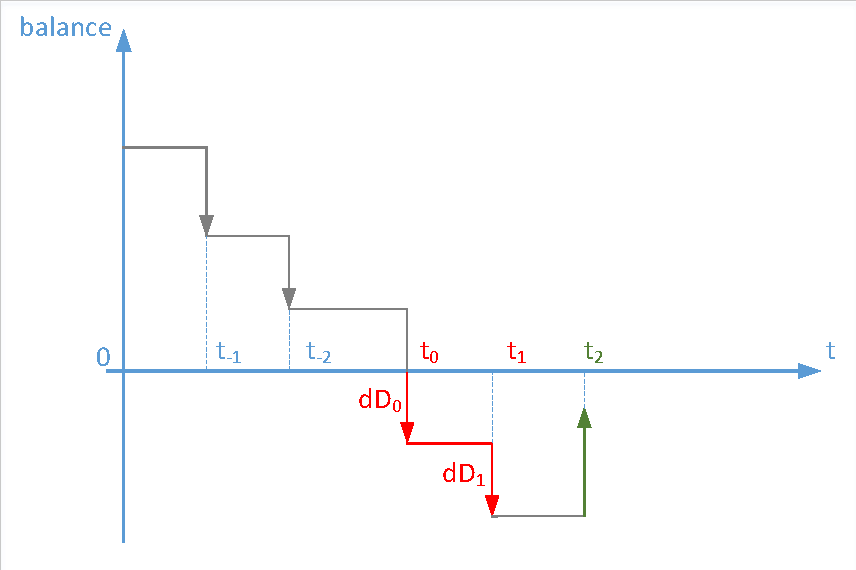
\includegraphics[width=0.5\textwidth, clip, trim=1mm 1mm 1mm 1mm]{Figures/deltadebt}
  \caption{\bf\small The delta debt progression}
  \label{fig:debt-graph}
\end{figure}

Figure \ref{fig:debt-graph} illustrates a transaction flow for a single account with 5 transactions and their timestamps named $t_i$, where $i$ covers the interval $[-2,2]$ in discrete steps of $1$. Two timestamps $t_j$ and $t_k$ having a $j>k$ imply that $t_j$ is older than $t_k$.

Let's assume a transaction as illustrated in the figure \ref{fig:debt-graph}, which turns a positive balance into a negative value. That event defines then a starting time stamp at $t_0$. This transaction creates a debt of $balance$ reduced by the transaction $amount$ given that $balance >=0$ and $amount > balance$. Debt will be handled further as a positive value, thus, we define a debt at position $i$

\begin{asm}
	debt_{t_i} = \left\{\begin{array}{ll}
           |balance_{t_i} - amount_{t_i}| \+ & \IF i = 0 \AND balance_{t_0} >= 0 \AND amount > balance\\
           amount_{t_i} & \ELSEIF i >= 0 \AND balance_{t_i} < 0
        \end{array}\right .\-
\end{asm}

When declaring $TXID_i$ as the transaction id we are defining a so called \textit{delta debt} as the following tuple

\begin{asm}
	dD_i = (t_i, TXID_i, Amount_{t_i}, DebtPos_{t_i})
\end{asm}

where the $Amount_{t_i}$ as well as $DebtPos_{t_i}$ are initialized with $debt_{t_i}$. In the following $Amount_{t_i}$ will always stay with its original value whereas $DebtPos_{t_i}$ will be reduced by an amount transferred \textbf{to} the same account.

\todo{asm code}